\documentclass{article}%ctex
\input{~/code/math_commands.tex}




\title{\huge Worksheet 3\\
\normalsize}
\author{Xuanxi Zhang}
\begin{document}
\maketitle



\section{Solving $Ax=b$ and LU factorization}
We will study the LU-factorization of the matrix
\begin{align*}
    A:=
  \begin{bmatrix}
    3  &   3   &    1\\
    6  &   4   &  9\\
    -6 &  -8   &   7
  \end{bmatrix}
\end{align*}
into the product
\begin{align*}
A = LU =
\begin{bmatrix}
1 & 0 & 0 \\
    \ell_{21} & 1 & 0\\
    \ell_{31} & \ell_{32} & 1
\end{bmatrix}
\begin{bmatrix}
    u_{11} & u_{12} & u_{13} \\
    0 & u_{22} & u_{23}\\
    0 & 0 & u_{33}
\end{bmatrix}
\end{align*}

\subsection{}
solve the $L$ and $U$ manully.

\subsection{}
show that the LU factorization is unique if A is non-singular. (Hint: Assume that $A=L_1U_1=L_2U_2$ and show that $L_1=L_2$ and $U_1=U_2$. Remember for lower  triangular matriices $L_1$ and $L_2$, $L_1^{-1}$  and $L_1\times L_2$ are also lower triangular matrices. )

\subsection{}\label{sec:3.1d}
Use the LU factorization to compute the determinant of
$A$. Recall that for two matrices of appropriate sizes,
$\det(AB)=\det(A)\det(B)$.

\subsection{}
In practical Gaussian elimination, the matrices $L_k$, are never formed and multiplied explicitly. The multipliers $\ell_{jk}$ are computed and stored directly into $L$, and the transformations $L_k$ are then applied implicitly.

\begin{enumerate}
    \item Verify that Gaussian elimination could be written as the following loop:
    \begin{figure}[H]
        \centering
        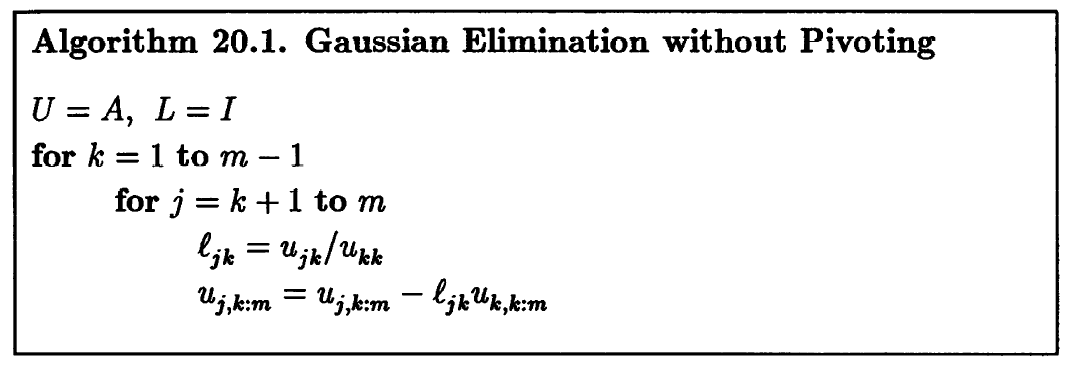
\includegraphics[width = 0.7\textwidth]{figs/TB97_Guass_wo_piv}
    \end{figure}
    \item Code this loop in MATLAB. Apply it to the matrix $A$ and obtain the $L$ and $U$ matrices.
\end{enumerate}

\subsection{}
Use the LU factorization to solve the linear system $Ax=b$ with
$b=[1, 0, 0]^\top$ using one forward and one backward substitution mannully. 

\subsection{}
check following code implamente forward substitution:
\lstinputlisting[
    caption=,
    label={},
    language=Matlab,
    ]{../code/MyForward.m}
try to code the forward and backward substitution in MATLAB.


  
\subsection{}
In the matrix $A$ defined above, replace the $(2,2)$-entry by $6$.
What is the rank of $A$ after this modification?
Attempt to compute the LU factorization of $A$. 
What do you observe?
How might you ``fix" the problem?


\section{Diagonally dominant matrix and pivoting}
A matrix is called strictly (column) diagonal-dominant if the
 the absolute value of the diagonal entry in each column is larger than
 the sum of the absolute values of the other entries in that
 column; i.e., for all $i$:
 $$
 |a_{ii}|>\sum_{j=1, j\not=i}^n |a_{ji}|
 $$
 
\subsection{}
Which of the following matrices is diagonally dominant?
$$
 B={\begin{bmatrix}-2&2&1\\1&3&2\\1&-2&0\end{bmatrix}}, \qquad
 C={\begin{bmatrix}-4&2&1\\1&6&2\\1&-2&5\end{bmatrix}}
$$

\subsection{}
When computing the LU
 factorization of a strictly diagonally dominant matrix, why is
 pivoting never necessary? 

\begin{enumerate}
    \item First argue why the first column does not require pivoting. Then use Gaussian elimination to generate the required zeros in the first column
    \item Show that, the submatrix you obtain when removing the first column and row is again strictly  diagonally dominant.
\end{enumerate}

\subsection{}
For diagonally dominant matrix, let's show that an LU decomposition without pivoting exists in a different way:
  \begin{enumerate}
    \item Why are the leading principal submatrices of a strictly
      diagonally dominant matrix also strictly diagonally dominant?
    \item Show that a diagonally dominant matrix is always invertible
      using the following argument: If $A$ is not invertible, then
      there must exists a vector $v\not=0$ such that
      $A v = \ve 0$. Call $r$ the largest (in
      absolute value) entry of $\ve v$ and consider
      multiplication of the $r$-th row. 
    \item Combine the previous two statements with a result from class
      to argue that the LU factorization of a strictly diagonally
      dominant matrix exists.
 \end{enumerate}

\section{Schur complement}
Assume $M\in \mathbb{R}^{(m+n)\times(m+n)}$ and we split them into blocks
\begin{align*}
    M = \begin{bmatrix}
    A &B\\
    C &D
    \end{bmatrix}
\end{align*}
where $A\in\mathbb{R}^{n\times n}$, $D\in\mathbb{R}^{m\times m}$, $B\in\mathbb{R}^{n\times m}$, and $C\in\mathbb{R}^{m\times n}$. We also assume that $M$ and all its leading submatrices are non-singular. 

\subsection{}
Verify the formula
\begin{align*}
     \begin{bmatrix}
    I & \\
    -CA^{-1} & I
    \end{bmatrix} \begin{bmatrix}
    A &B\\
    C &D
    \end{bmatrix} =  \begin{bmatrix}
    A &B\\
     &D-CA^{-1}B
    \end{bmatrix}
\end{align*}
for ``elimination" of the block $C$. The matrix $D-CA^{-1}B$ is  known as the \textit{Schur complement} of $A$ in $M$.









\end{document}